
\documentclass[compress,aspectratio=43]{beamer}

\usepackage{fontspec}
\usepackage{polyglossia}
\setmainlanguage{english}
\usepackage[english]{isodate}
\isodate
\usepackage{multicol}
\usepackage{feynmp-auto}
\usepackage{siunitx}
\sisetup{separate-uncertainty}
\usepackage{booktabs}
\usepackage{biblatex}
\addbibresource{main.bib}

\usetheme{vertex}

\linespread{1.3}

\title{Search for $B\to D\mu\mu$}
\subtitle{Theory and Analysis outline}
\date{\today}
\institute{Very Rare Decays WG Meeting}
\author[Igor Babuschkin]{\small \textbf{Igor Babuschkin} \and Julian Wishahi \and Alex Shires \and Johannes Albrecht}

\begin{document}

\maketitle

\begin{frame}{The decay $B^0\to\overline{D}^0\mu^+\mu^-$}
  \centering
  \begin{columns}
    \begin{column}{0.35\textwidth}
      \begin{fmffile}{b2dmumu}
        \centering
        \unitlength=1mm
        \begin{fmfgraph*}(40, 25)
          \fmfcmd{%
            vardef cross_bar (expr p, len, ang) =
            ((-len/2,0)--(len/2,0))
              rotated (ang + angle direction length(p)/2 of p)
              shifted point length(p)/2 of p
            enddef;
            style_def crossed_before expr p =
              cdraw p;
              cfill (harrow (p, .4));
              ccutdraw cross_bar (p, 4mm, 45);
              ccutdraw cross_bar (p, 4mm, -45)
            enddef;
            style_def crossed_after expr p =
              cdraw p;
              cfill (harrow (p, .9));
              ccutdraw cross_bar (p, 4mm, 45);
              ccutdraw cross_bar (p, 4mm, -45)
            enddef;
            style_def crossed_wiggly expr p =
              cdraw (wiggly p);
              ccutdraw cross_bar (p, 4mm, 45);
              ccutdraw cross_bar (p, 4mm, -45)
            enddef; }
          \fmfleft{i1,i2}
          \fmfright{o1,o2}
          \fmf{crossed_after}{v1,i1}
          \fmf{crossed_before}{o1,v1}
          \fmf{crossed_before}{i2,v2}
          \fmf{crossed_after}{v2,o2}
          \fmf{boson,label=$W$}{v1,v2}
          \fmfv{label=$b$}{i1}
          \fmfv{label=$c$}{o1}
          \fmfv{label=$d$}{i2}
          \fmfv{label=$u$}{o2}
        \end{fmfgraph*}

        \centering
        \vspace{3em}
        \begin{fmfgraph*}(20, 15)
          \fmfleft{i1}
          \fmfright{o1,o2}
          \fmf{photon}{i1,v1}
          \fmf{fermion}{o1,v1,o2}
          \fmfv{label=$\gamma/Z^0$,decoration.size=0.2w,decoration.shape=cross}{i1}
          \fmfv{label=$\mu$}{o2}
          \fmfv{label=$\mu$}{o1}
        \end{fmfgraph*}

      \end{fmffile}
    \end{column}
    \begin{column}{0.70\textwidth}
      \begin{itemize}
        \item $W$ exchange (no penguin loop)
        % Why is this decay interesting?
        \item Two conflicting theoretical predictions:
        \item Evans et al. [1999] ($q^2 > \SI{1}{GeV}$)\\ $\mathrm{BR}(B^0\to \overline{D}^0 e^+e^-) = 2.6\times10^{-9}$
        \item Kim et al. [2011] ($q^2 \in [1,5]\,\si{GeV}$) \\ $\mathrm{BR}(B^0\to \overline{D}^0 \mu^+\mu^-) = \left(9.7^{+4.2}_{-3.2}\right)\times10^{-6}$
      \end{itemize}
    \end{column}
  \end{columns}
\end{frame}

\begin{frame}{Evans et al.}
  \begin{itemize}
    \item Use effective field theory to separate decay into short/long distance interactions
    \item In absence of lattice QCD calculations, matrix elements $β$ and $β_8$ must be approximated
    \item Also gave predictions for $B^+->D_(s)^{(*)+}e^+e^-$ (smaller BR) in a different paper
  \end{itemize}
\end{frame}

\begin{frame}{Kim et al.}
  \begin{itemize}
    \item Perturbative QCD approach
    \item Make use of model-dependent \enquote{wave functions} to derive result
    \item No mention of calculation by Evans et al.
  \end{itemize}
\end{frame}

\begin{frame}{Expected number of candidates}
  \begin{columns}
    \begin{column}{0.4\textwidth}
      \begin{itemize}
        \item $\mathcal{L} = \SI{3.189}{\per\femto\barn}$
        \item $σ_{b\overline{b}} = \SI{295 \pm 29}{\micro\barn}$
        \item $f_d \approx \num{0.4}$
        \item $ε_\text{geom} \approx \num{0.15}$
        \item $ε_\text{trig} \approx \num{0.8}$
        \item $ε_\text{strip} \approx \num{0.2}$
      \end{itemize}
    \end{column}
    \begin{column}{0.7\textwidth}
      \begin{itemize}
        \item $\mathrm{BR}(D^{0}\to K^-\pi^+) = \SI{3.87 \pm 0.05}{\percent}$
        \item $\mathrm{BR}(D^+\to K^-\pi^+\pi^+) = \SI{9.13 \pm 0.19}{\percent}$
        \item $\mathrm{BR}(D_s^+\to K^+K^-\pi^+) = \SI{5.49 \pm 0.27}{\percent}$
        \item $\mathrm{BR}(D^{*0} \to D^0\pi^0) = \SI{61.9 \pm 2.9}{\percent}$
        \item $\mathrm{BR}(D^{*+} \to D^0\pi^+) = \SI{67.7 \pm 0.5}{\percent}$
        \item $\mathrm{BR}(D_s^{+*}\to D_s^+\pi^0) = \SI{5.8 \pm 0.7}{\percent}$
        \item Looked at \cite{evans1}\cite{evans2} for $B$ decay BRs
        \item (All $B$ BRs for $q^2 > \SI{1}{GeV^2}$)
      \end{itemize}
    \end{column}
  \end{columns}
\end{frame}

\begin{frame}{Expected number of candidates (cont.)}
  \centering
  \begin{tabular}{l S S}
    \toprule
    Decay & {\text{Predicted BR}} \cite{evans1}\cite{evans2} & {\text{Expected yield}} \\
    \midrule
    $B^0\to \overline{D}^0\mu\mu$ & 2.6e-9 & 1.8 \\
    $B^0\to \overline{D}^{*0}\mu\mu$ & 1.4e-8 & 6.1 \\
    $B^+\to D^+\mu\mu$ & 2.5e-12 & 0.41e-2 \\
    $B^+\to D^{+*}\mu\mu$ & 1.0e-11 & 0.48e-2 \\
    $B^+\to D_s^+\mu\mu$ & 4.3e-11 & 0.17e-2 \\
    $B^+\to D_s^{+*}\mu\mu$ & 2.0e-10 & 0.12e-1 \\
    $B_c\to D_s^+\mu\mu$ & ? & ? \\
    $B_c\to D_s^{*+}\mu\mu$ & ? & ? \\
    \bottomrule
  \end{tabular}
\end{frame}

\begin{frame}{Trigger and Stripping}
  \begin{itemize}
    \item TODO: List trigger lines
  \end{itemize}
  \begin{itemize}
    \item Stripping line: \texttt{StrippingB2XMuMu\_Line}
    \item TODO: List stripping cuts here
  \end{itemize}
\end{frame}

\begin{frame}{Preparation: Blind signal region, Remove $J/\psi$}
  \centering
  \includegraphics[width=0.75\textwidth,page=80]{../../../plots/select.pdf}
\end{frame}

\begin{frame}{Preselection}
  \begin{itemize}
    \item {\small Cut on PID variables and \texttt{isMuonLoose} to select Kaon/Pion:}
    \item {\small Resample PID variables from data for MC}
  \end{itemize}
  \centering
  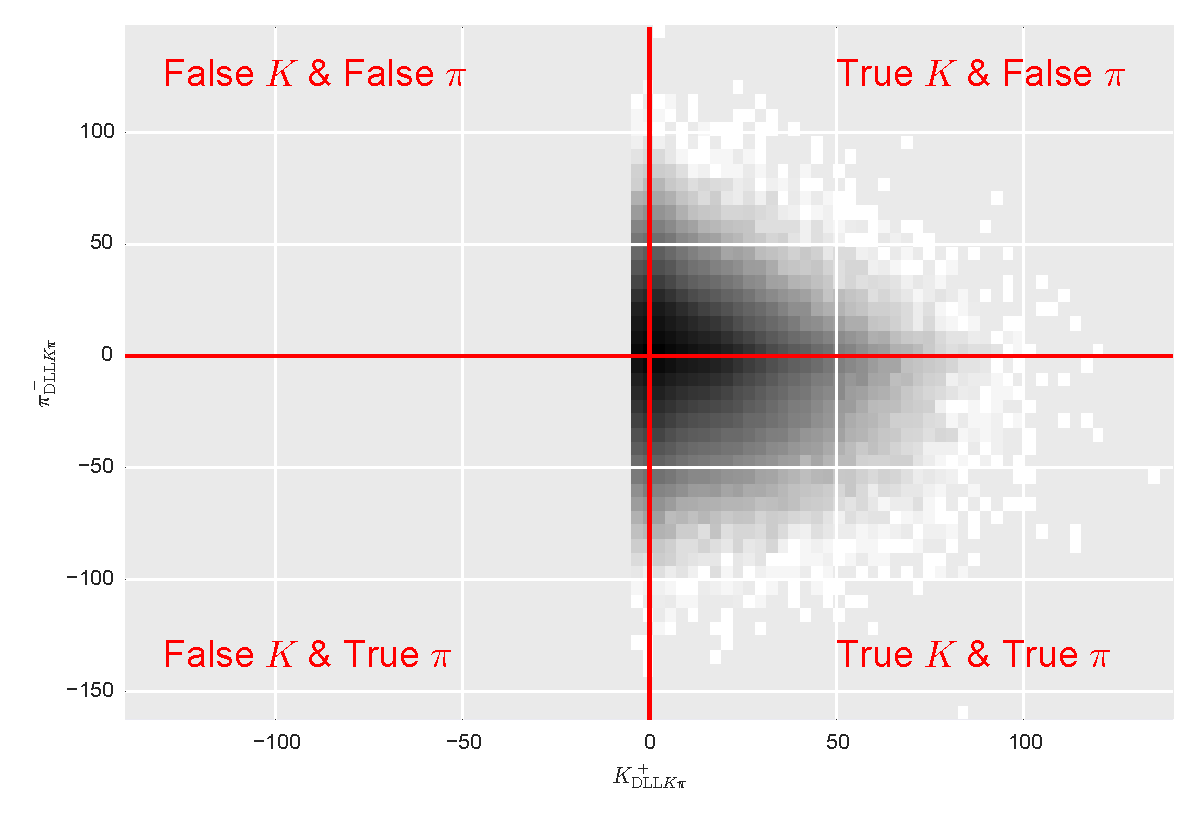
\includegraphics[width=0.8\textwidth]{../../../plots/pid_plot.pdf}
\end{frame}

\begin{frame}{Multivariate selection: variables}
  \begin{itemize}
    \item Currently: mostly kinematic variables
    \item Also: Isolation discriminant used for $B^0\to K^{*0}\mu\mu$
  \end{itemize}
  \centering
  \includegraphics[trim=0 0 0 7em,clip,width=0.7\textwidth]{../../../plots/correlation.pdf}
\end{frame}

\begin{frame}{Multivariate selection: cross-validation}
  \begin{itemize}
    \item Use $k$-fold validation to assess quality of classifier (BDT):
  \end{itemize}
  \centering
  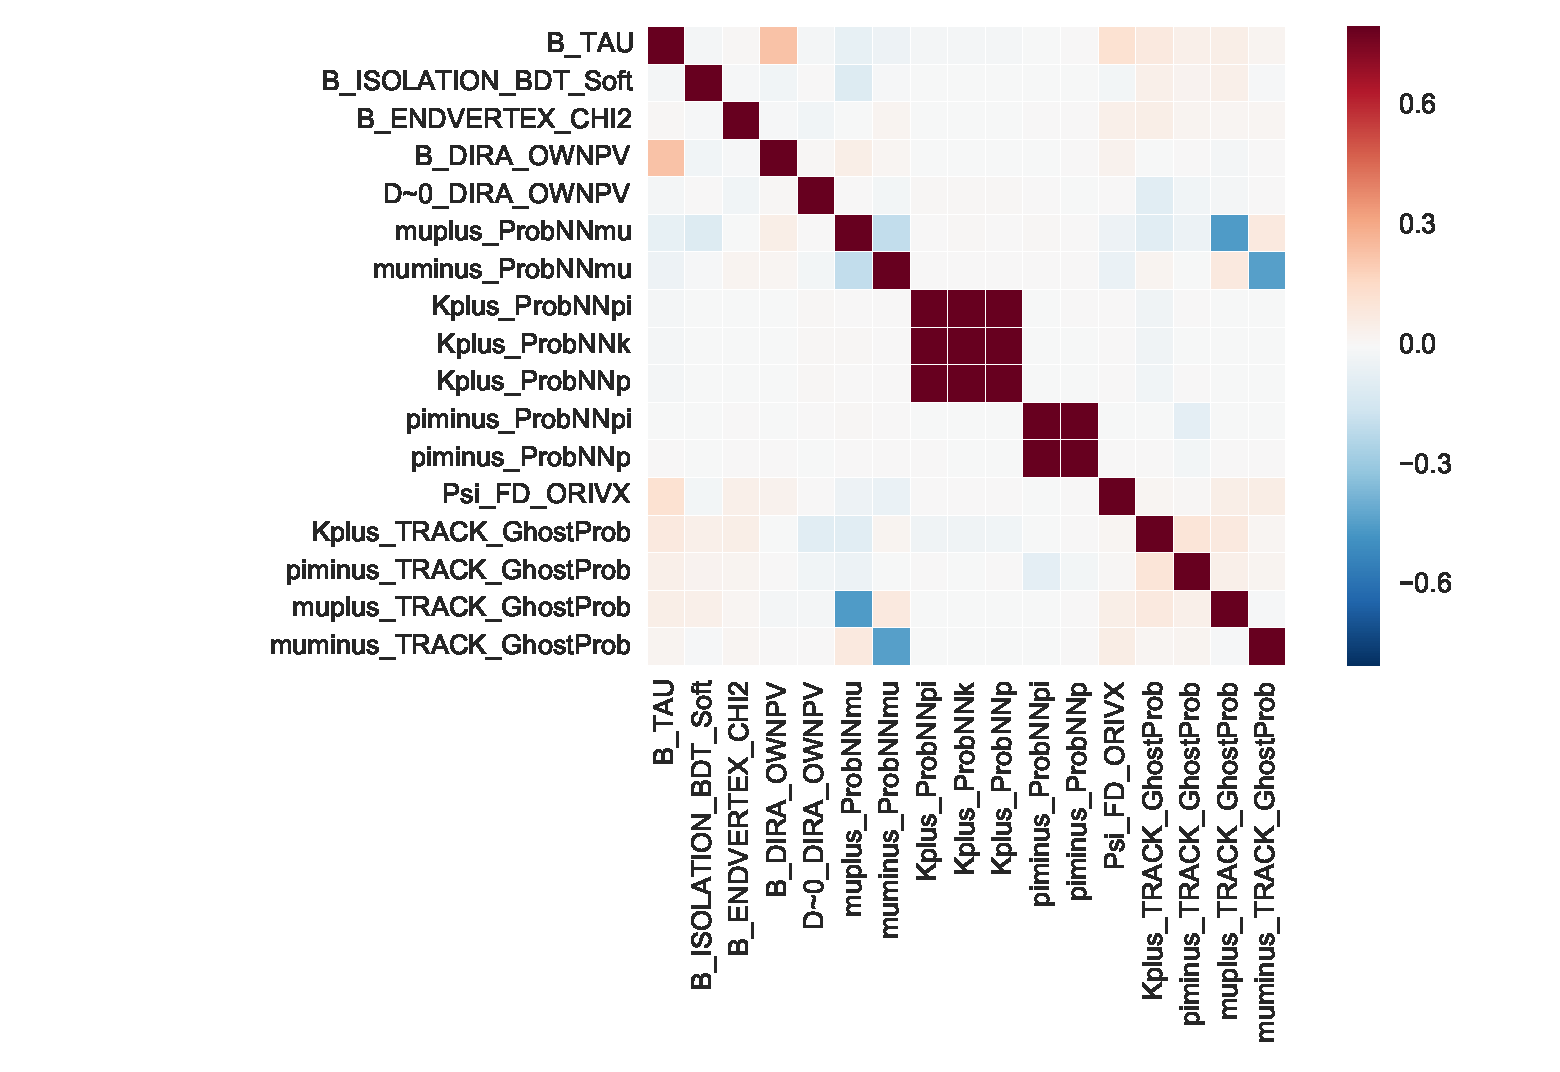
\includegraphics[width=0.65\textwidth,page=1]{../../../plots/classifier.pdf}
\end{frame}

\begin{frame}{Multivariate selection: partial dependence on $B^0$ mass}
  \centering
  \includegraphics[width=\textwidth]{../../../plots/classifier_mass.pdf}
\end{frame}

\begin{frame}{Statistical model}
  \begin{itemize}
    \item Currently in development
    \item Suspected problem: $B^0\to K^+\pi^-\mu^+\mu^-$ peaking under signal
      \begin{itemize}
        \item Idea: Include $D^0$ mass (and optionally $D^0$ decay time) into fit 
      \end{itemize}
    \item Infer signal mass shape from simulation
    \item First goal: Build model and fit Toy MC:
  \end{itemize}
  \centering
  \includegraphics[width=0.70\textwidth,trim=0 0 0 4em,clip]{../../../plots/fit.pdf}
\end{frame}

\begin{frame}{Measurement of branching fraction}
  Efficencies to take into account:
  \begin{itemize}
    \item trigger efficiency (use TISTOS on control channel)
    \item stripping efficiency (how?, MC?)
    \item LHCb acceptance efficency
    \item preselection efficiency (use PIDCalib?)
    \item selection efficiency of BDT
  \end{itemize}
  $\Rightarrow$ Use signal yield and efficiencies to derive BR estimate.
  \begin{itemize}
    \item Use normalization channel, but which one?
  \end{itemize}
\end{frame}

\begin{frame}{Systematic uncertainties}
  \begin{itemize}
    \item TODO
  \end{itemize}
\end{frame}

\begin{frame}{Outlook}
  \begin{itemize}
    \item Analysis of $B^0\to \overline{D}^0 \mu\mu$ is progressing well
    \item Will be extended to look at the resonant mode $B^0\to J/\psi\overline{D}^0$ (same dataset, currently not observed)
    \item Could be extended to other modes (e.g. $B^+\to D^{*+}\mu\mu$, $B^+\to D_s^+\mu\mu$)
  \end{itemize}
  Judging from theory predictions (Evans): Expect to set limits
  \begin{itemize}
    \item But: The BR could be underestimated!
  \end{itemize}
\end{frame}

\begin{frame}{Bibliography}
  \small
  \printbibliography
\end{frame}

\end{document}

